% -----------------------------------------------------------------------------------------------------
% A3. Sources: results/A3_summary.json (rho_lemma; speed-ups speedup_exact_over_lemma and speedup_exact_over_rho, with
% rho = min{sigma/(6 theta_1), theta_1/(2n)}; r_var, r_cen, r_coco_lk, c_share, q_cancel, maximal violation; sign-aware
% keys contraction_componentwise_max, q_plus_frac_ge_1, q_cancel_frac_ge_1_given_inner_positive,
% c_share_frac_negative_given_q_ge_1), digest.md A3 tables, A3 note (Thm. lk, Lemma L1, Prop. cancel, eq. cancel,
% predictions (P2)-(P4), outcome paragraph), findings.md Secs. 5 and 8. B3 speed-ups on the same logistic problems:
% digest. Computed from results/A3.pkl (records before Psi < 1e-10, as in the summary): the speed-ups over passes 2-20.
% Growth from kappa = 1e3 to 1e4 on logistic regression: 4.117/2.775 = 1.48 for L-Katyusha (A3_summary.json, key
% speedup_exact_over_lemma) and 15.73/5.155 = 3.05 for SAGA (B3_summary.json, attribution, key speedup).
% -----------------------------------------------------------------------------------------------------
\subsection{The Lyapunov proof of L-Katyusha, measured (hypothesis A3)}\label{sec:exp-A3}

Appendix~\ref{sec:lkatyusha} reproduces the proof of~\cite{kovalev2020dont} in the style of the book, which gives
\resref{thm:lk}, restated in Section~\ref{sec:th-A3}. We measure its one-step contraction~\eqref{ineq:contraction}
(Lemma~10 of~\cite{kovalev2020dont}), $\Ei[\Psi_{t+1}]\le c_ZZ_t+c_YY_t+c_WW_t$ with $c_Z$, $c_Y$, $c_W$ the three
coefficients of \resref*{thm:lk}, exactly along L-Katyusha runs on (H) with $m=64$ and $\kappa=10^4$ ($\theta_1=0.033$)
and on logistic regression with $\alpha=1$ and $\kappa=10^3$ ($\theta_1=\frac12$) or $10^4$ ($\theta_1=0.26$)
(Figure~\ref{fig:A3}). All statistics of this section pool the instrumented states of the three seeds from $t=0$ until
$\Psi_t$ first falls below $10^{-10}$ or the run ends, i.e.\ over the first 16 to 60 passes. The contraction is never
violated: the largest value of $(\Ei[\Psi_{t+1}]-c_ZZ_t-c_YY_t-c_WW_t)/\Psi_t$ over all recorded states is
$-6.5\cdot10^{-4}$, $-2.3\cdot10^{-4}$ and $-1.7\cdot10^{-4}$, and that of its consequence
$\rho_{\rm exact}(t)-\max\{c_Z,c_Y,c_W\}$, with $\rho_{\rm exact}(t)=\Ei[\Psi_{t+1}]/\Psi_t$, is $-1.7\cdot10^{-3}$,
$-4.0\cdot10^{-4}$ and $-2.8\cdot10^{-4}$. The exact one-step contraction exponent exceeds the certified one, that of
$\max\{c_Z,c_Y,c_W\}$, by a factor $4.7$, $2.8$ and $4.1$ ($5.9$, $2.8$ and $4.1$ over passes 2--20, the window used for
SAGA), against $5.2$ and $15.7$ for SAGA and Proposition~\ref{prop:59} on the same logistic problems. The closed-form rate
$\rho$ of~\eqref{ineq:rate} in \resref*{thm:lk} gives away a further factor $\frac43$ at $\kappa=10^3$ and $2$ on the two
problems with $\kappa\ge\frac{8n}3$ (through $\frac1{1+x}\le1-\frac x2$): against it the factors are $9.3$, $3.7$ and
$8.2$. The variance bound~\eqref{ineq:var} of \resref{lem:L1}, $\Ei\norm{g_t-\Fp(x_t)}^2\le2L\,D_F(w_t,x_t)$, has
tightness $0.125$--$0.15$ (geometric means; maxima $0.30$--$0.59$): its centering step~\eqref{ineq:var-center} is nearly
tight ($0.94$--$0.99$) and the slack is in its cocoercivity step~\eqref{ineq:var-coco} ($0.13$--$0.15$), which uses the
worst-case curvature $L=\max_iL_i$ for gradient differences along $w_t-x_t$, where the curvature met is far smaller (on
(H) all $L_i$ are equal, so this is not a max-versus-average effect), as for I2. The signed share
$c(t)=\inner{\Fp(x_t)}{x_t-w_t}/D_F(w_t,x_t)$ of the Bregman gap that the anchor removes in the identity~\eqref{eq:cancel}
of \resref{prop:cancel} is negative on $77\%$, $77\%$ and $64\%$ of the steps (medians $-1.5$, $-0.61$, $-0.62$) and above
$1$ on $12\%$, $8\%$ and $20\%$: the cancelled inner product is rarely a fraction of the gap, which illustrates why the
proof cancels it identically rather than bounding it. Its size relative to the certified one-step decrease, $q(t)$, has
medians $1.4$, $0.64$ and $1.4$, and $q(t)\ge1$ on $63\%$, $5\%$ and $65\%$ of the steps.

\begin{figure}[tbp]
  \renewcommand{\thefigure}{A3}% project figure name (see the header of this file)
  \centering
  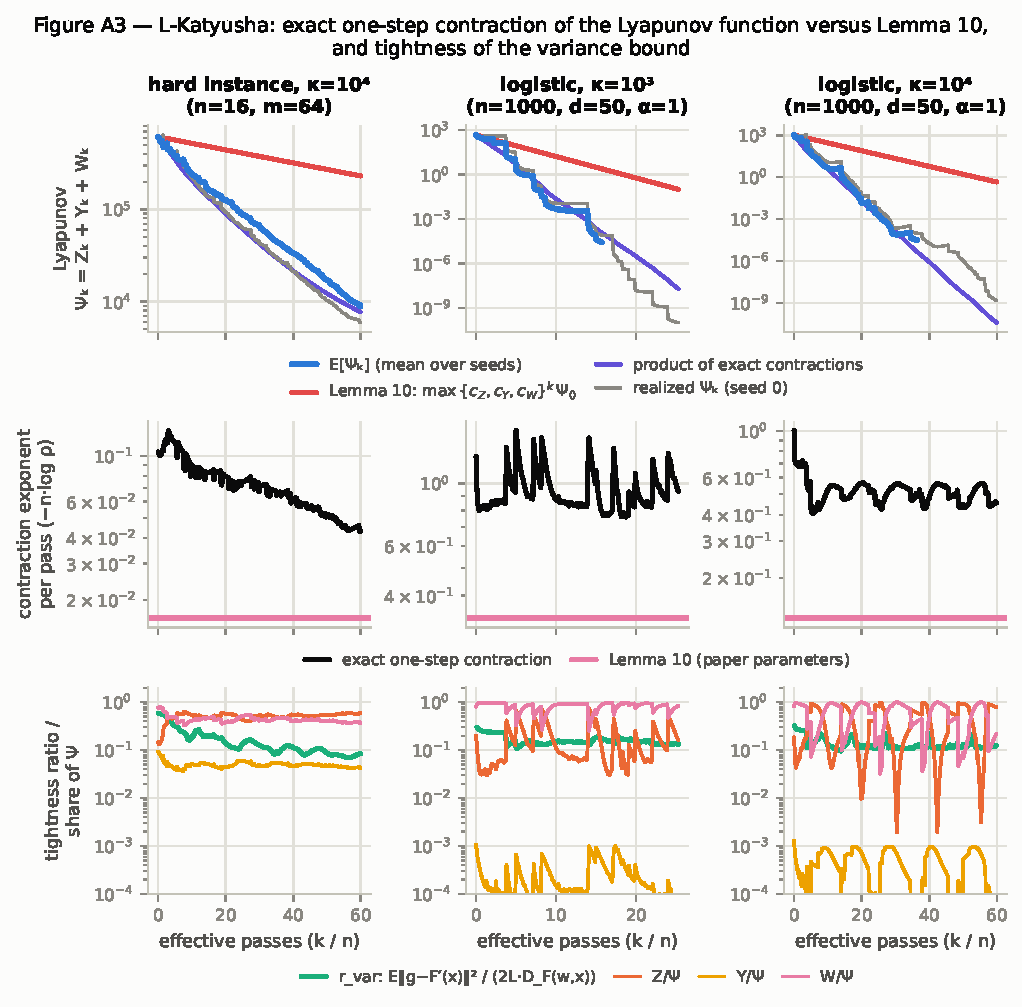
\includegraphics[width=\textwidth]{figA3_lkatyusha_lyapunov}
  \caption{\textbf{Hypothesis A3: the Lyapunov proof of L-Katyusha, measured.} L-Katyusha with the parameters of
  Theorem~11 of~\cite{kovalev2020dont} ($\theta_2=\frac12$, $\theta_1=\min\{\sqrt{2n/(3\kappa)},\frac12\}$, $p=\frac1n$) on (H)
  ($n=16$, $m=64$, $\kappa=10^4$) and on logistic regression ($n=1{,}000$, $d=50$, $\alpha=1$, $\kappa\in\{10^3,10^4\}$),
  3 seeds, records with $\Psi_t<10^{-10}$ discarded (the iteration counter is written $k$ in the figure). Top: the
  Lyapunov function $\Psi_t=Z_t+Y_t+W_t$ (mean over seeds), the contraction $\max\{c_Z,c_Y,c_W\}^t\Psi_0$ certified by
  Lemma~10 of~\cite{kovalev2020dont} (inequality~\eqref{ineq:contraction}), the product of the exact conditional
  contractions along seed $0$ and the realized $\Psi_t$ of seed $0$. Middle: exact one-step contraction exponent per pass
  along seed $0$ against the certified one. Bottom (seed $0$): tightness of the variance bound
  $\E\norm{g-\Fp(x)}^2\le2L\,D_F(w,x)$ and shares of $Z$, $Y$ and $W$ in $\Psi$.}
  \label{fig:A3}
\end{figure}

The proof thus holds along the trajectories. Its looseness ($2.8$ and $4.1$ at $\kappa=10^3$ and $10^4$ on logistic
regression, $4.7$ on (H)) is smaller than that of Proposition~\ref{prop:59} on the same logistic problems ($5.2$ and
$15.7$) and grows less between these two values of $\kappa$ ($\times1.5$ against $\times3.1$); two values of $\kappa$, in
different regimes of the certificate ($c_W$ binding at $\kappa=10^3$, where $\theta_1=\frac12$, and $c_Z$ at $10^4$), do not
determine how it scales. Both certificates have the optimal order in the worst case, by the lower bounds of
Section~\ref{sec:th-A1} for L-Katyusha and by \resref{prop:B3-lower} for SAGA, so the difference concerns these instances,
not the order of the bounds. On the two ill-conditioned problems the cancelled term exceeds the whole certified decrease
on about two thirds of the steps, as the part of prediction (P4) of Section~\ref{sec:lk-naive} on L-Katyusha anticipates.
On most of these steps, however, it has the favourable sign ($c(t)<0$ on $84\%$ and $70\%$ of them, against none of the
$5\%$ of such steps at $\kappa=10^3$): if $c(t)\le0$, then $D_F(w_t,x_t)\le F(w_t)-F(x_t)$, a difference of function values,
which a reference potential can pay. The sign-aware ratio $q_+(t)$, which counts the cancelled term only where $c(t)>0$, is
at least $1$ on $9.9\%$, $5.2\%$ and $19.3\%$ of the recorded states, that is, on $43\%$, $23\%$ and $54\%$ of the states
with $c(t)>0$: only there could the cancelled term not have been absorbed into the certified decrease, which is the
mechanism behind predictions (P2) and (P3) of Section~\ref{sec:lk-naive} for the naive scheme.

% -----------------------------------------------------------------------------------------------------
% A2. Sources: results/A2_summary.json and digest.md A2 tables (one seed; gradients to 1e-10 for the trajectories, read at
% the first record below the target, to 1e-6 for the grid, interpolated log-linearly between records by
% vrlab.algorithms.grads_to_accuracy; counts in units of n as in the titles and cells of Figure A2); counts with stored
% reference gradients: grad_evals - iters at the stop in results/A2.pkl; A3 note (Def. naive, Rem. naive-book, Props.
% naive, naive-kappa, prediction (P2)); findings.md Sec. 6; Allen-Zhu Sec. 7.1 as quoted in the A3 note and in the
% related-work section. Dimension condition (ineq:dim) for kappa = 1e4, at 1e-6 and 1e-10: right-hand sides 86.4 and
% 143.9 (144.0 in the sqrt form) with Q = 1 + (kappa - 1)/n; 108.3 and 180.6, i.e. m >= 109 and m >= 181, with
% q = 0.93823 for Q_b = 1 + 4c/mu_b = 984.47 of (H) (q + 1/q = 2 + mu_b/c, c = 245.87 from
% vrlab.problems.make_hard_instance(16, 64, 1e4)); q^(2m) = 2.9e-4 at m = 64 (q^(2m) = 1.04e-6 > 1e-6 at m = 108).
% -----------------------------------------------------------------------------------------------------
\subsection{Naive acceleration (hypothesis A2)}\label{sec:exp-A2}

What happens when Nesterov's momentum is combined with the loopless-SVRG estimator $g=\fip(x)-\fip(w)+\Fp(w)$ without the
negative momentum of Katyusha? We test L-Katyusha with $\theta_2=0$ and the same $\theta_1$, $\eta$, $p$, that is, the
scheme of \resref{def:naive} with $\eta=1/(3\theta_1)$, and the two-sequence form
$v=\theta+\beta(\theta-\theta_{\rm prev})$, $\theta^+=v-\gamma g(v)$, with the reference point reset to $v$ with
probability $\frac1n$, tuned over $\beta\in\{0.5,0.8,0.9,0.95,(\sqrt\kappa-1)/(\sqrt\kappa+1)\}$ and
$\gamma R^2\in\{\frac16,\frac1{20},\frac1{60}\}$ (best setting: fewest gradients to the relative error $10^{-6}$). The
latter is a variant of \resref*{def:naive} without the drift term of \resref{rem:naive-book}, with the reference point
reset to the query point instead of the gradient-step iterate, and with $(\beta,\gamma)$ free; \resref{prop:naive} and
\resref{prop:naive-kappa} are proved for \resref*{def:naive} only. Both schemes are compared with SAGA, L-SVRG, L-Katyusha
with the untuned parameters of its theorem, and AGD, on (H) with $m=64$, $\kappa=10^4$, and on logistic regression with
$\kappa=10^4$, $\alpha=1$ (one seed each, Figure~\ref{fig:A2}). With $m=64$, the analogue for (H) of the dimension
condition~\eqref{ineq:dim} of \resref{cor:count}, $q^{2m}\le\varepsilon$ with $q=(\sqrt{Q_b}-1)/(\sqrt{Q_b}+1)=0.938$ and
$Q_b=1+4c/\mu_b$ (Section~\ref{sec:setting}), fails at the accuracies $10^{-6}$ and $10^{-10}$ used here, which need
$m\ge109$ and $m\ge181$: the lower bound is not certified on this instance, and the certified window is explored with
$m=256$ in Section~\ref{sec:exp-A4}.

\begin{figure}[tbp]
  \renewcommand{\thefigure}{A2}% project figure name (see the header of this file)
  \centering
  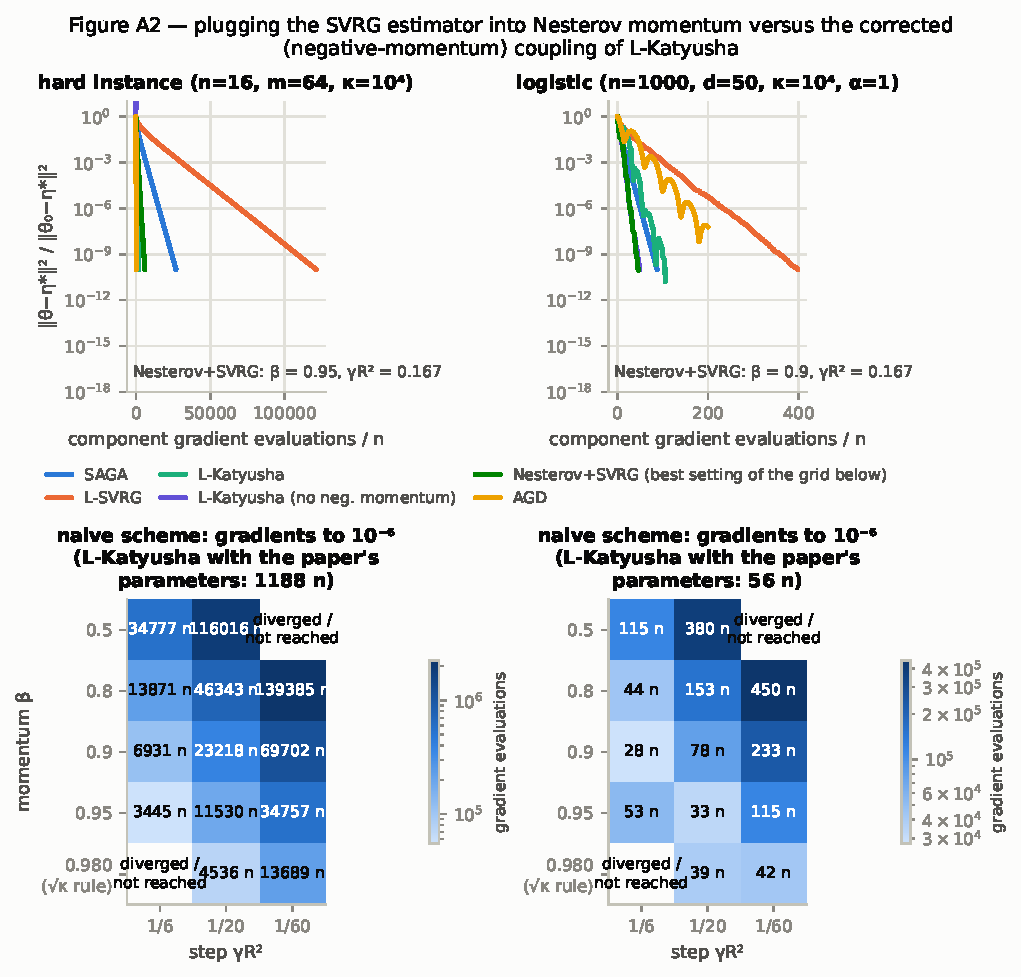
\includegraphics[width=\textwidth]{figA2_naive_acceleration}
  \caption{\textbf{Hypothesis A2: naive acceleration.} Top: relative error $\norm{\theta-\etastar}^2/\norm{\theta_0-\etastar}^2$
  (for L-Katyusha, $\theta=y_t$) against component gradient evaluations (counted as in Section~\ref{sec:exp-protocol})
  divided by $n$, for SAGA, L-SVRG, L-Katyusha (parameters of Theorem~11 of~\cite{kovalev2020dont}), L-Katyusha without
  the negative-momentum term ($\theta_2=0$), Nesterov momentum applied to the loopless-SVRG estimator (best setting of the
  grid below, given in each panel) and AGD, on (H) ($n=16$, $m=64$, $\kappa=10^4$) and on logistic regression ($n=1{,}000$, $d=50$,
  $\kappa=10^4$, $\alpha=1$); one seed, runs stopped at the first record below $10^{-10}$. Bottom: gradient evaluations needed
  by the naive scheme to reach the relative error $10^{-6}$ (interpolated log-linearly between records) for each
  $(\beta,\gamma R^2)\in\{0.5,0.8,0.9,0.95,(\sqrt\kappa-1)/(\sqrt\kappa+1)\}\times\{\frac16,\frac1{20},\frac1{60}\}$ (white cells:
  divergence or budget exhausted); the titles give the count of L-Katyusha with its untuned parameters.}
  \label{fig:A2}
\end{figure}

On (H), reaching $10^{-10}$ (counts read at the first record below the target) costs $5.3\cdot10^3$ gradients to AGD,
$3.2\cdot10^4$ to L-Katyusha, $9.6\cdot10^4$ to the best naive setting ($\beta=0.95$, $\gamma R^2=\frac16$),
$4.3\cdot10^5$ to SAGA and $1.9\cdot10^6$ to L-SVRG, while L-Katyusha with $\theta_2=0$ diverges (relative error
$8.8\cdot10^{27}$ after $3.4\cdot10^3$ gradients). With the rule $\beta=(\sqrt\kappa-1)/(\sqrt\kappa+1)=0.980$ the naive
scheme diverges at $\gamma R^2=\frac16$ and needs $4536n$ and $13\,689n$ gradients to reach $10^{-6}$ at
$\gamma R^2=\frac1{20}$ and $\frac1{60}$, against $1188n$ for L-Katyusha; the best setting of the grid needs $3445n$,
$2.9$ times more. AGD is the cheapest here because $L_F=R^2/n$ (Section~\ref{sec:exp-A4}). On logistic regression the
order of AGD, L-Katyusha and the best naive setting is reversed: reaching $10^{-10}$ costs $4.7\cdot10^4$ gradients to the
best naive setting ($\beta=0.9$, $\gamma R^2=\frac16$), $4.9\cdot10^4$ to L-Katyusha with $\theta_2=0$, $8.8\cdot10^4$ to
SAGA, $1.06\cdot10^5$ to L-Katyusha ($7.1\cdot10^4$, fewer than SAGA, with stored reference gradients) and $4.0\cdot10^5$
to L-SVRG, while AGD ($L_F/\mu=654$) is still at $6.1\cdot10^{-8}$ after 200 passes; to $10^{-6}$, the best naive setting
needs $28n$ against $56n$ for L-Katyusha, and the $\sqrt\kappa$ rule fails at $\gamma R^2=\frac16$ (final relative error
$1.26$ after 200 passes) and needs $39n$ and $42n$ at the smaller steps.

On (H) the negative momentum is what keeps the coupling stable: removing it produces the divergence anticipated by
prediction (P2) of Section~\ref{sec:lk-naive} for $\kappa\gg n$, and the momentum scheme must be detuned, which costs it
the advantage over L-Katyusha. \resref{prop:naive} and \resref{prop:naive-kappa} describe the same obstruction in the
proof, for the scheme of \resref{def:naive}: without the anchor the one-step inequality keeps the uncontrolled term
$\frac\nu{\theta_1}D_F(w_t,x_t)$, and closing it with smoothness and strong convexity costs a factor $\kappa$. On a benign
logistic problem, whose effective constants are much better than the worst-case ones ($\muEff\approx5\mu$ near $\etastar$
and $\LEff\approx R^2/9$ along SAGA, Section~\ref{sec:exp-B2}), the anchor-free schemes converge and are about twice as
fast as L-Katyusha with worst-case parameters ($\theta_1=\sqrt{2n/(3\kappa)}=0.26$), in line with the report
of~\cite[Section~7.1]{allenzhu2018katyusha} that the scheme without negative momentum is sometimes faster after careful
tuning but does not accelerate on some tasks. These observations come from two instances, one seed and a grid that favours
the naive scheme (fifteen settings against an untuned L-Katyusha); they do not show that it cannot accelerate, a question
that no lower bound known to us settles, as noted in \resref{rem:naive-honest}.
